\documentclass{article}
\usepackage[utf8]{inputenc}

\title{Pagina03}

\begin{document}

\section{Paso 15:} 
\begin{itemize}
	\item Ahora seguiremos con la instalacion dejaremos que instale para luego poder logearnos con nuestro codigo.
	\begin{center}
	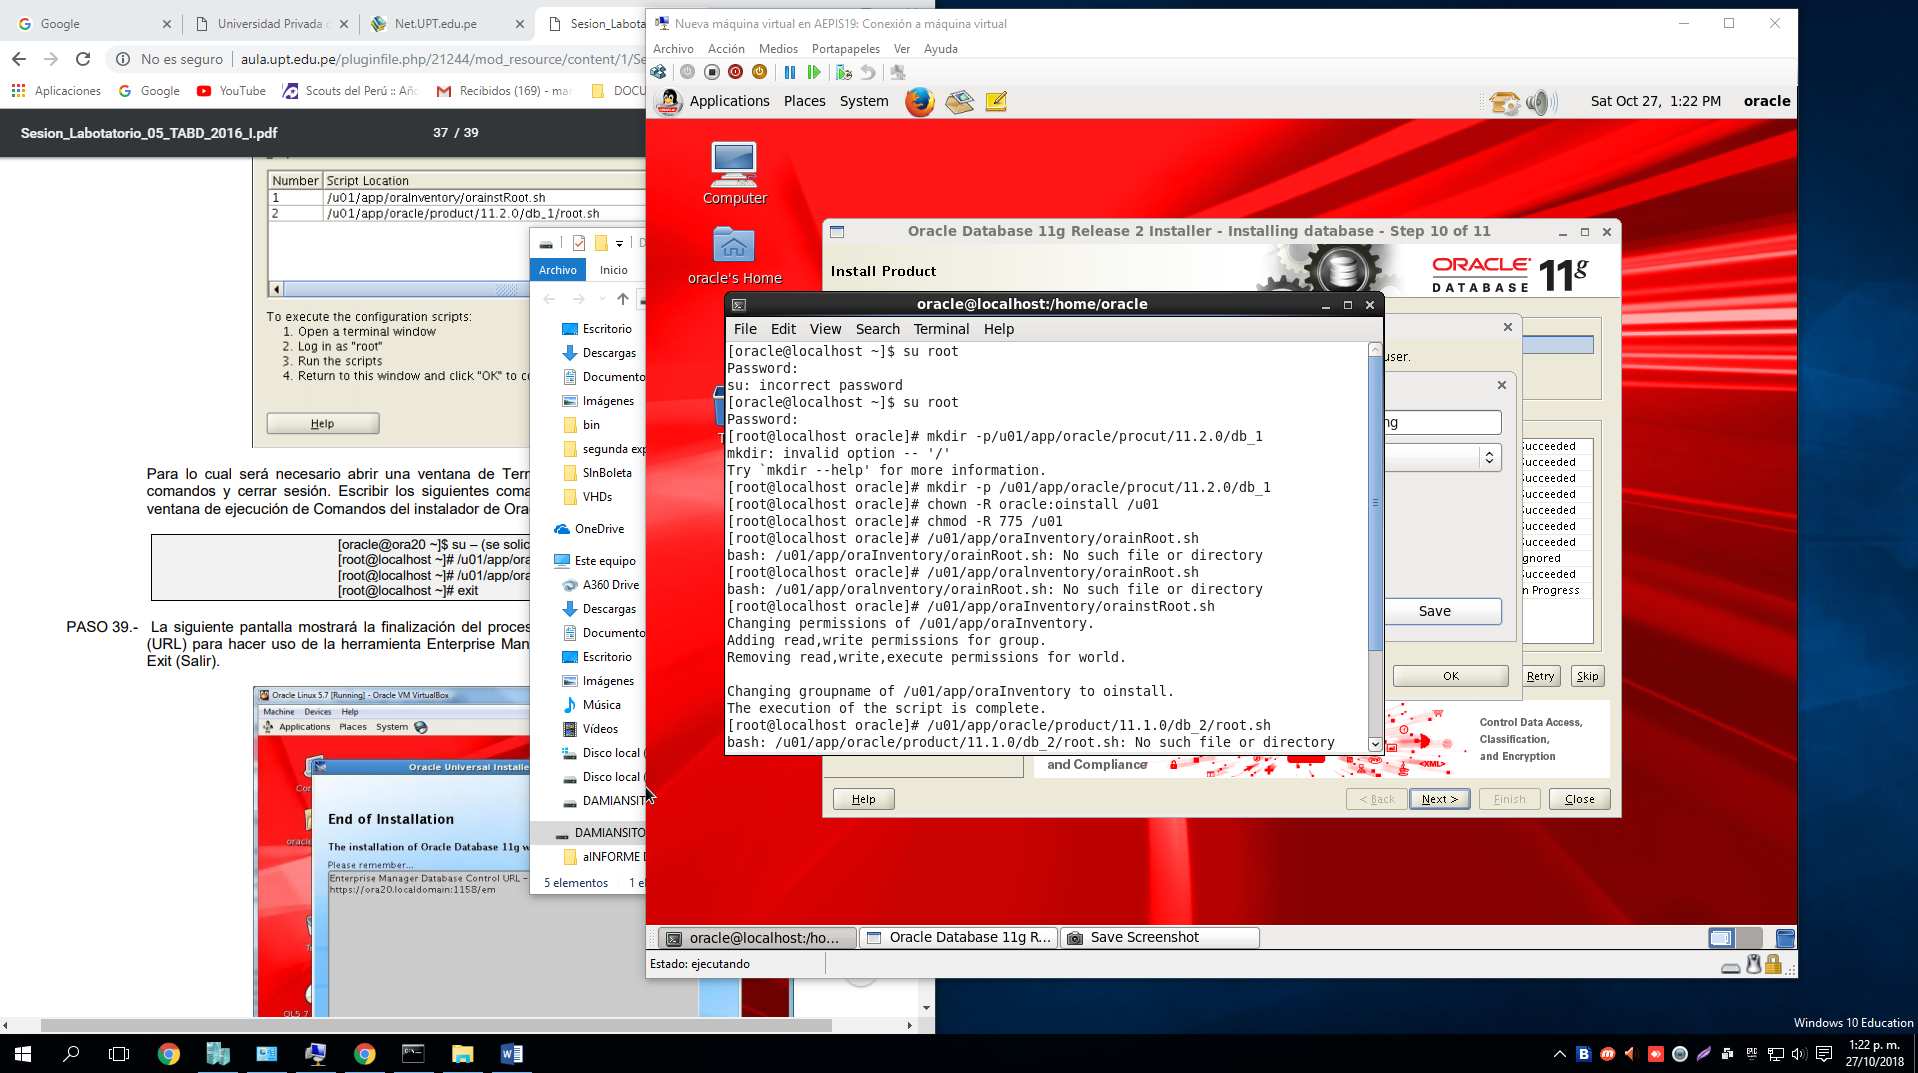
\includegraphics[width=14cm]{./Imagenes/imagen15} 
	\end{center}
	
\section{Paso 16:}
	\item Ahora seguidamente damos siguiente hasta llegar a este punto de finish, para luego dar close y termina la instalacion.
	\begin{center}
	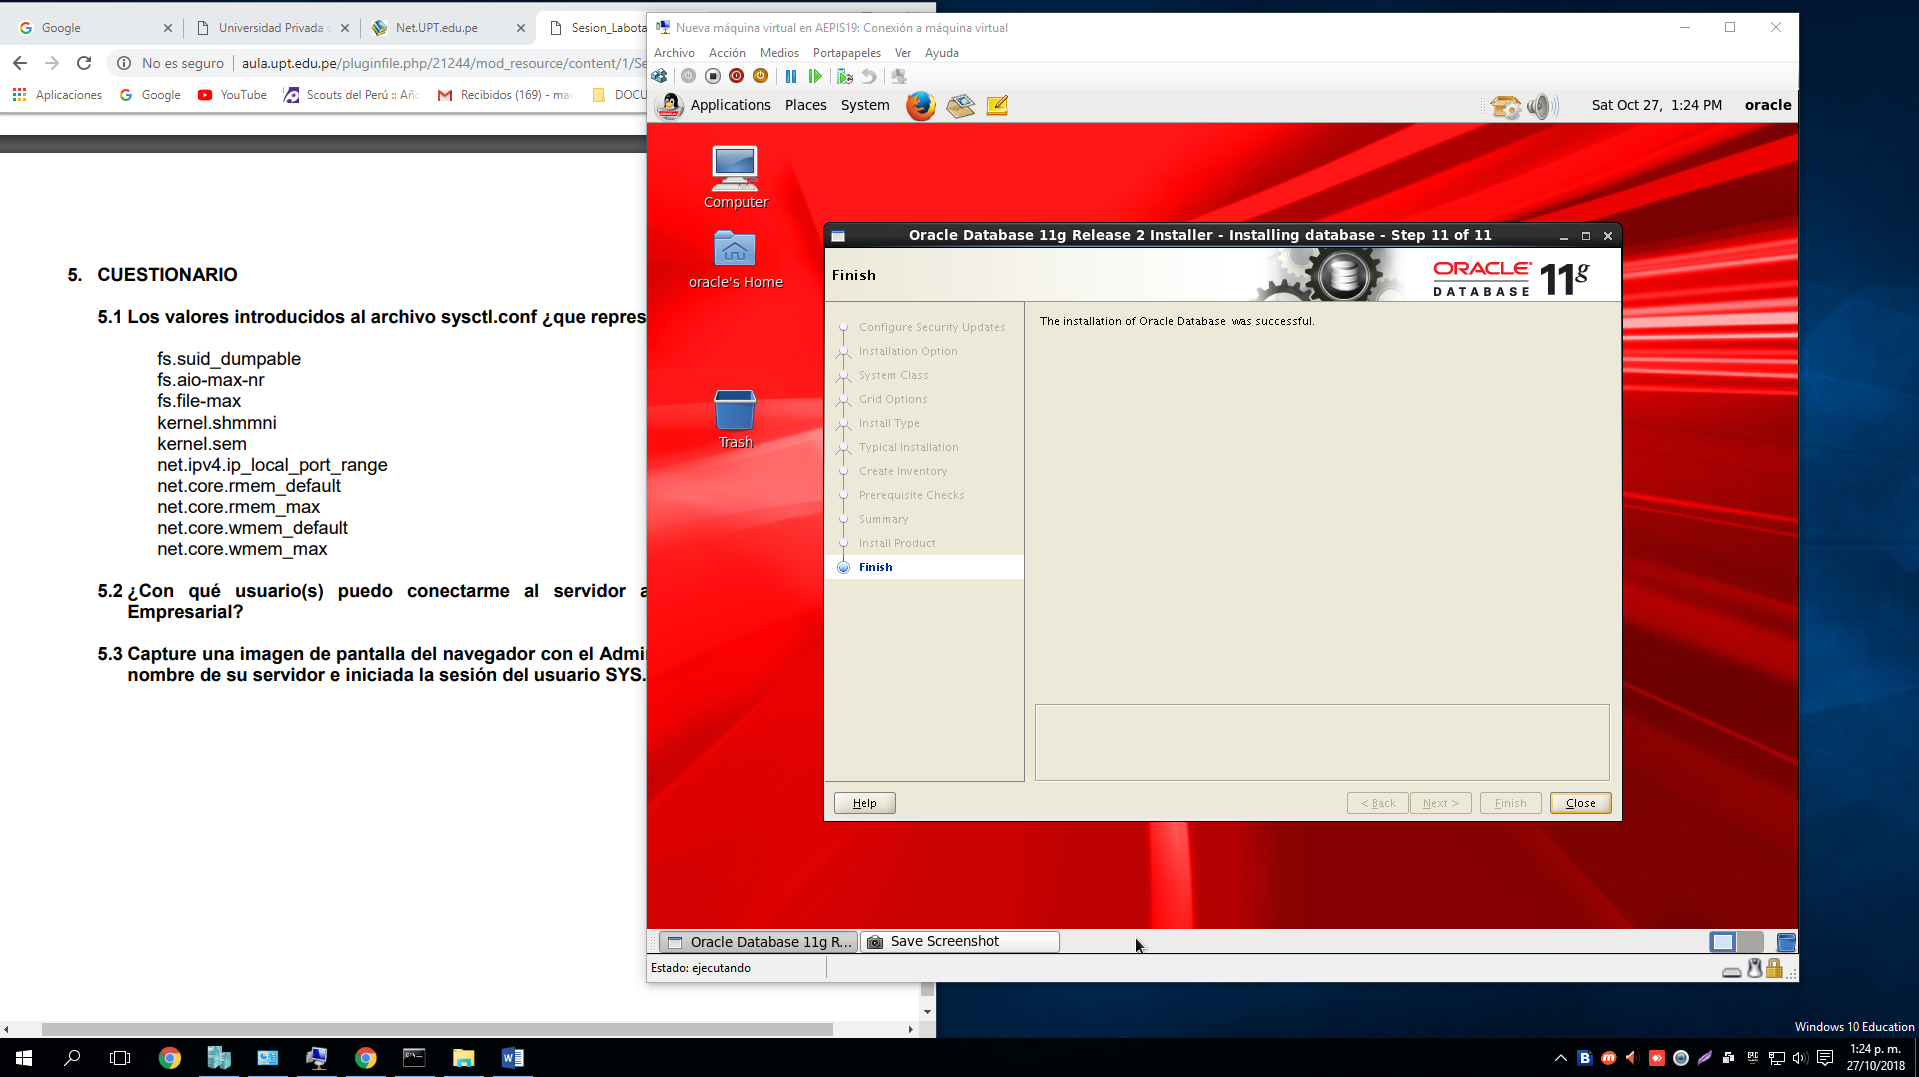
\includegraphics[width=14cm]{./Imagenes/imagen16} 
	\end{center}
\newpage
\section{Paso 17:} 
	\item Ahora reiniciamos la maquina virtual, mirando el ping de la maquina virtal, para su uso correcto.
	\begin{center}
	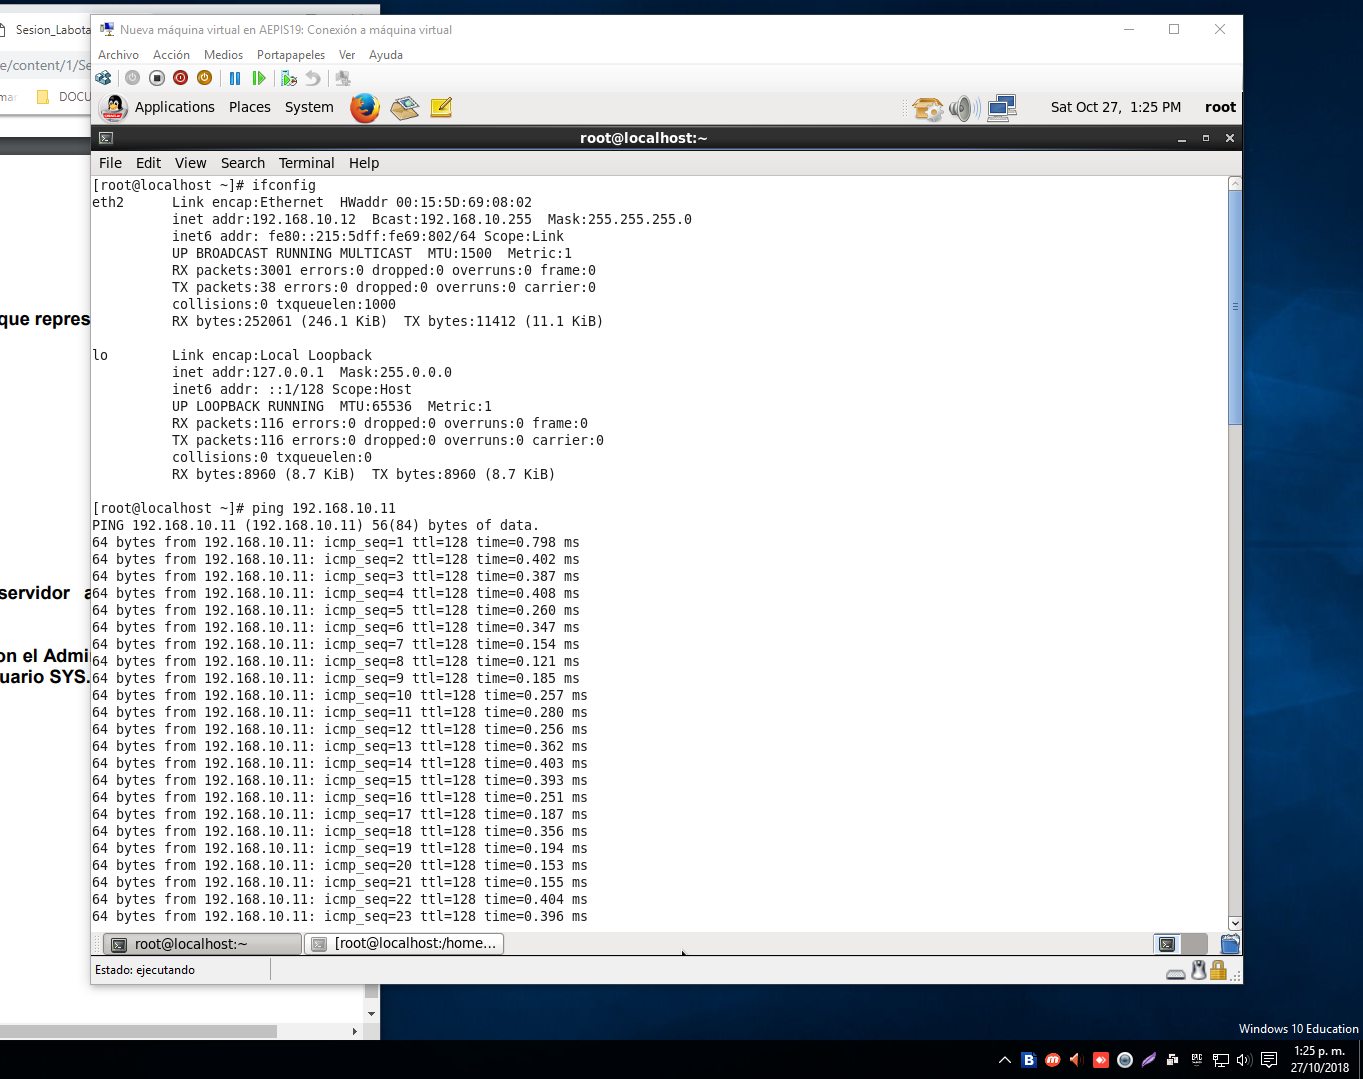
\includegraphics[width=14cm]{./Imagenes/imagen17} 
	\end{center}
\section{Paso 18:} 
	\item Seguidamente buscamos el cd de oracle para que el funionamiento esa correcto.
	\begin{center}
	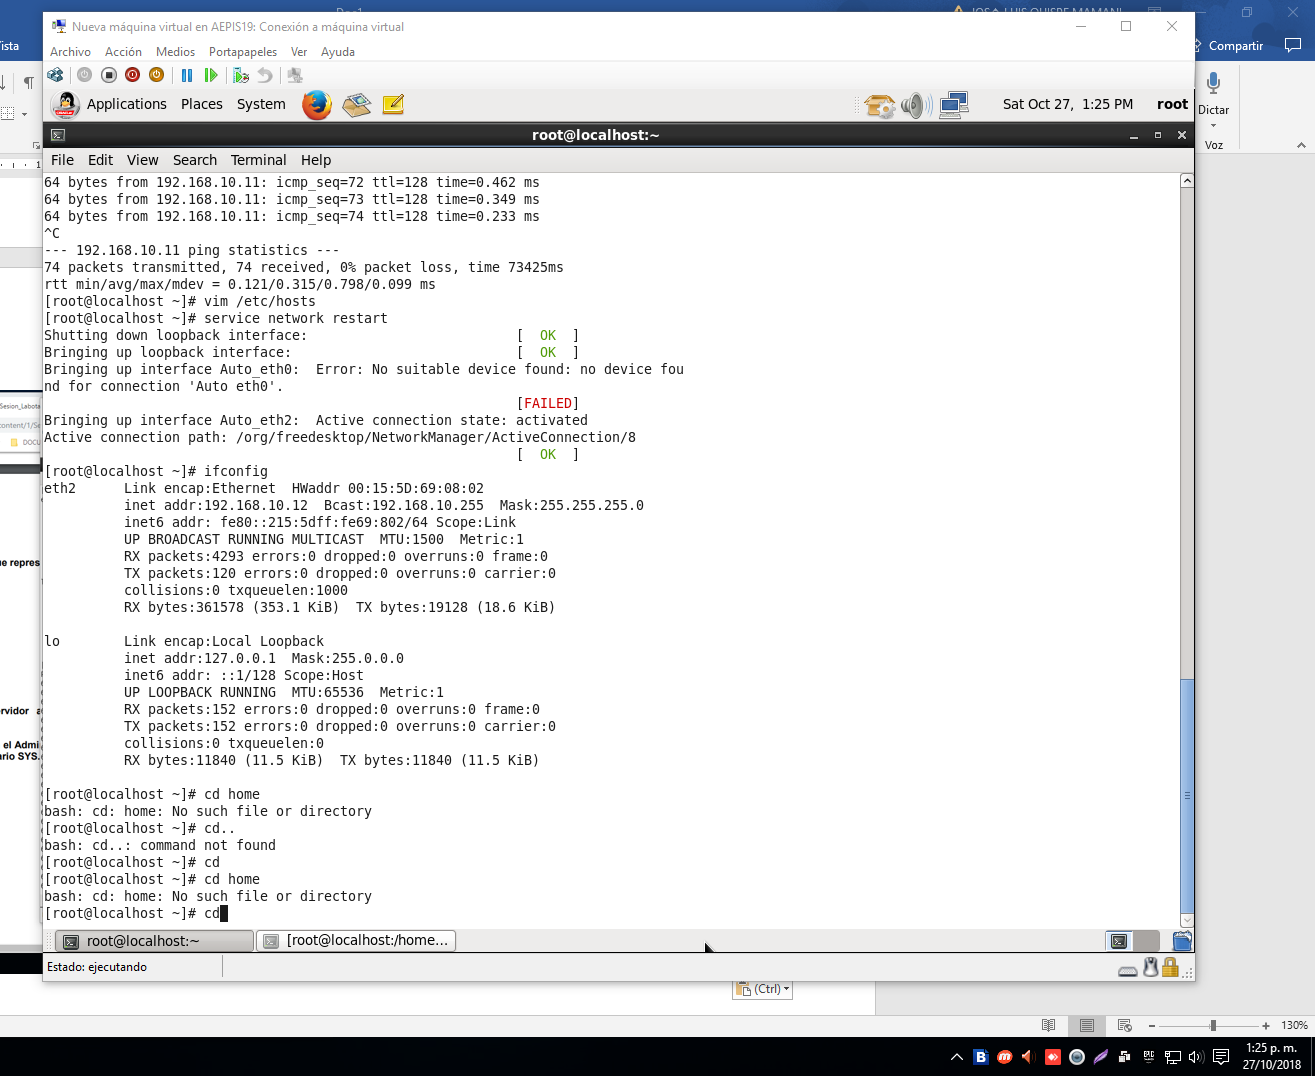
\includegraphics[width=14cm]{./Imagenes/imagen18} 
	\end{center}
\newpage
\section{Paso 19:} 
	\item Continuamos con la instalacion la parte del cd oracle.
	\begin{center}
	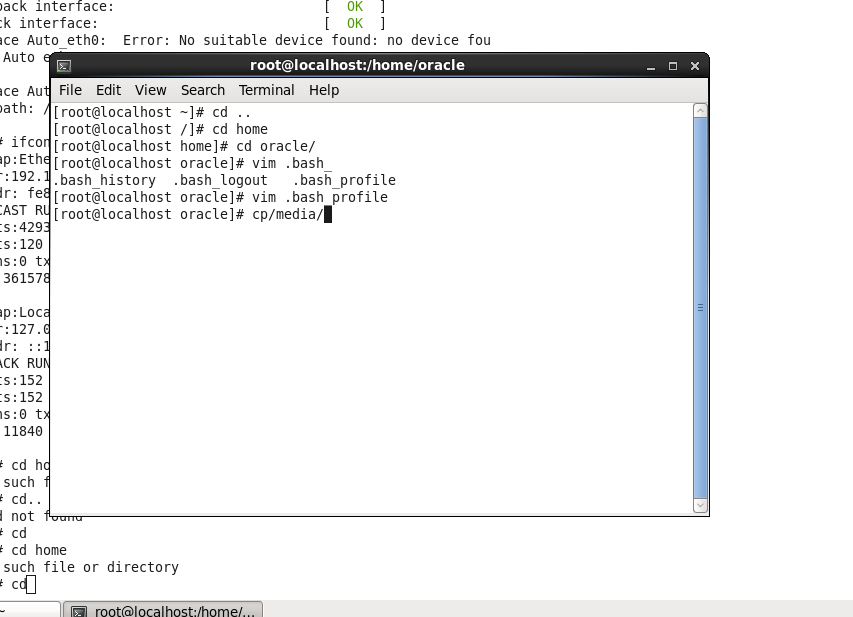
\includegraphics[width=13cm]{./Imagenes/imagen19} 
	\end{center}

\section{Paso 20:}
	\item continuando con la instalacion del Oracle.
	\begin{center}
	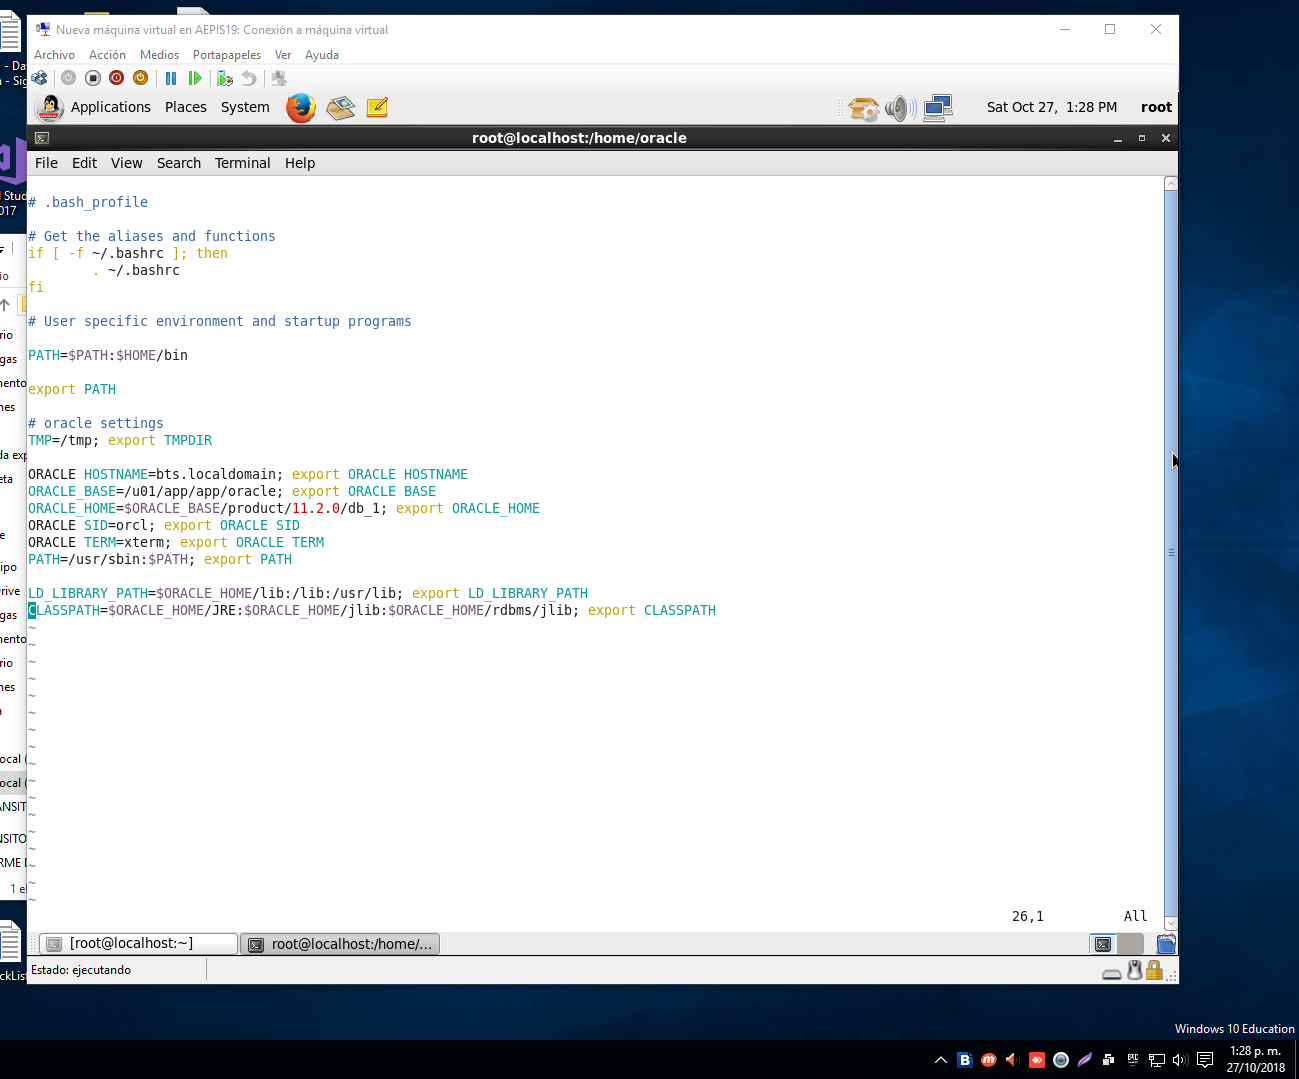
\includegraphics[width=13cm]{./Imagenes/imagen20} 
	\end{center}
	
\newpage
\section{Paso 21:}
	\item continuando con la instalacion del Oracle.
	\begin{center}
	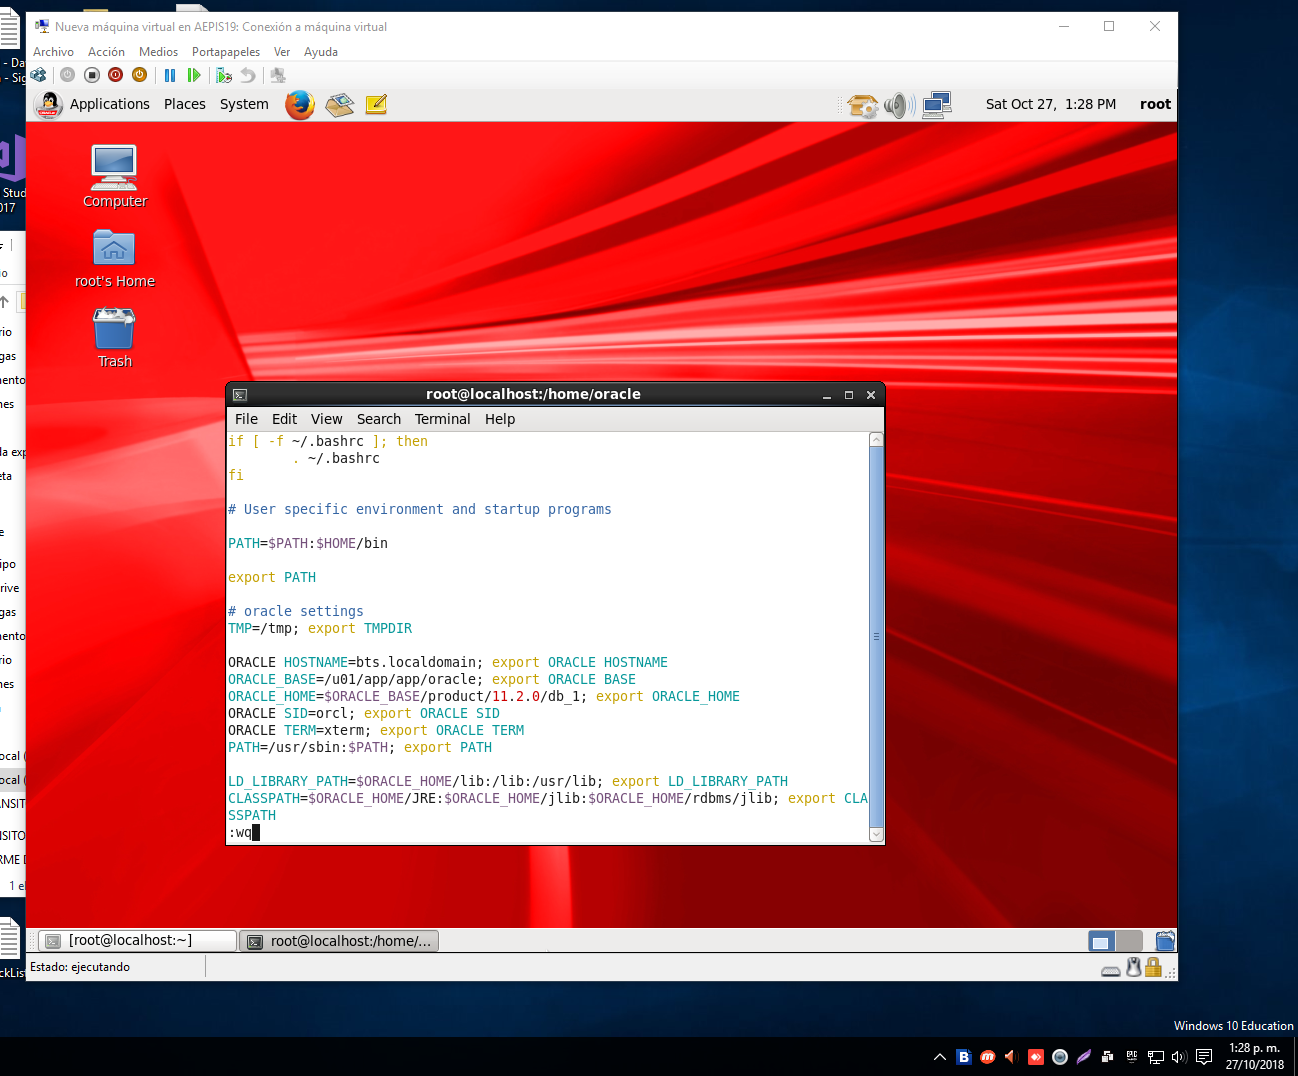
\includegraphics[width=13cm]{./Imagenes/imagen21} 
	\end{center}

\section{Paso 22:}
	\item En este paso vamos sistema de archivos. 
	\begin{center}
	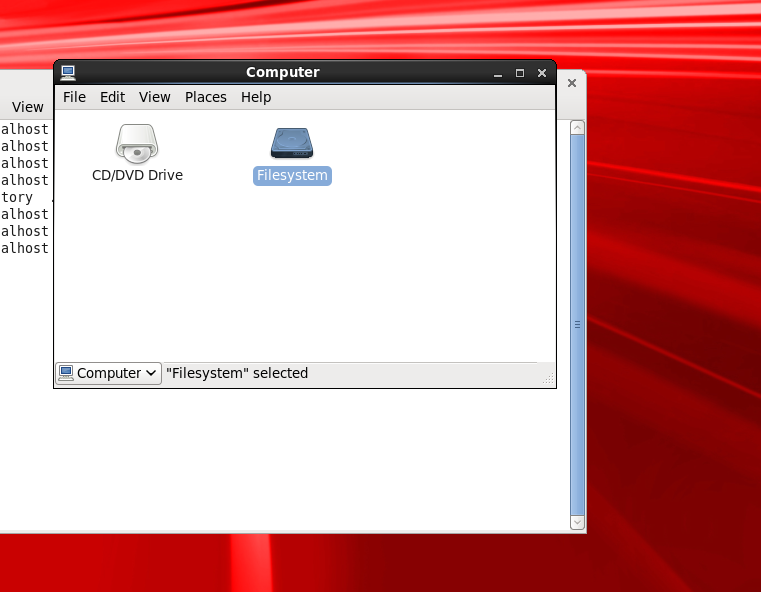
\includegraphics[width=13cm]{./Imagenes/imagen22} 
	\end{center}
	
	
\newpage
\section{Paso 23:}
	\item continuando con la instalacion del Oracle.
	\begin{center}
	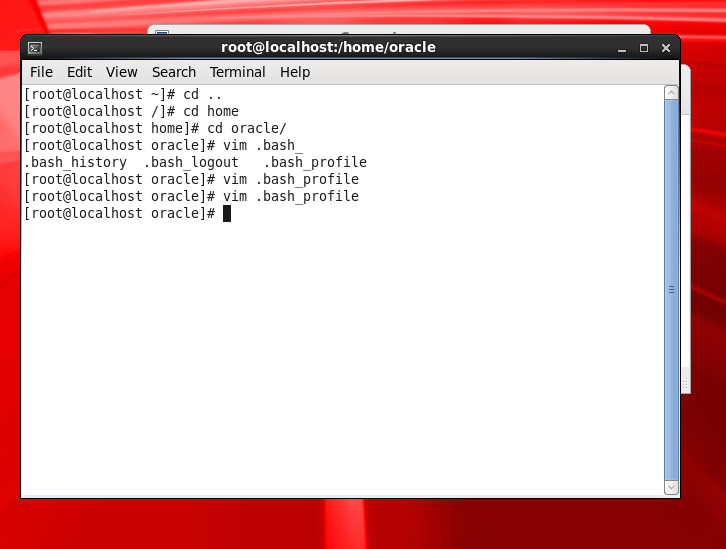
\includegraphics[width=13cm]{./Imagenes/imagen23} 
	\end{center}

\end{itemize} 
\end{document}
